\documentclass[final,hyperref={pdfpagelabels=false}]{beamer}
\usepackage{grffile}
\mode<presentation>{\usetheme{I6pd2}}
\usepackage[english]{babel}
\usepackage[latin1]{inputenc}
\usepackage{amsmath,amsthm, amssymb, latexsym}
%\usepackage{times}\usefonttheme{professionalfonts}  % obsolete
%\usefonttheme[onlymath]{serif}
\boldmath
\usepackage[orientation=portrait,size=a0,scale=1.4,debug]{beamerposter}
\usepackage{ragged2e} 
\usepackage{bm}
% change list indention level
% \setdefaultleftmargin{3em}{}{}{}{}{}

%\usepackage{snapshot} % will write a .dep file with all dependencies, allows for easy bundling


\usepackage{array,booktabs,tabularx}
\newcolumntype{R}{>{\raggedleft\arraybackslash}X} % right justified tabularx columns
\newcommand{\pphantom}{\textcolor{ta3aluminium}} % phantom introduces a vertical space in p formatted table columns??!!
\newcommand{\p}{\partial}
\newcommand{\bu}{\bm{u}}
\newcommand{\bv}{\bm{v}}

\listfiles

%%%%%%%%%%%%%%%%%%%%%%%%%%%%%%%%%%%%%%%%%%%%%%%%%%%%%%%%%%%%%%%%%%%%%%%%%%%%%%%%%%%%%%
\graphicspath{{figures/}}
 
\title{\huge Gap formation and stability in non-isothermal
  disks\\ \Large [2014 CITA Summer Student Program]}
\author{Min-Kai Lin and Robert Les}
\institute[CITA]{Canadian Institute for Theoretical Astrophysics, 60
  St George Street, Toronto, M5S 3H8, Canada}
%% \date[Sep. 8th, 2009]{Sep. 8th, 2009}

%%%%%%%%%%%%%%%%%%%%%%%%%%%%%%%%%%%%%%%%%%%%%%%%%%%%%%%%%%%%%%%%%%%%%%%%%%%%%%%%%%%%%%
\newlength{\columnheight}
\setlength{\columnheight}{105cm}
\setbeamertemplate{caption}{\centering\insertcaption\par}

%%%%%%%%%%%%%%%%%%%%%%%%%%%%%%%%%%%%%%%%%%%%%%%%%%%%%%%%%%%%%%%%%%%%%%%%%%%%%%%%%%%%%%
\begin{document}
\begin{frame}
  \begin{columns}
    % ---------------------------------------------------------%
    % Set up a column 
    \begin{column}{.49\textwidth}
      \begin{beamercolorbox}[center,wd=\textwidth]{postercolumn}
        \begin{minipage}[T]{.95\textwidth}  % tweaks the width, makes a new \textwidth
          \parbox[t][\columnheight]{\textwidth}{ % must be some better way to set the the height, width and textwidth simultaneously
            % Since all columns are the same length, it is all nice and tidy.  You have to get the height empirically
            % ---------------------------------------------------------%
            % fill each column with content            
            \begin{block}{{\Large Introduction}}
              \justifying
                  {\large              
                    {\bf
                    }
                  }
            \end{block}
            \vfill
            
            \begin{block}{{\Large Disk-planet model with simple cooling}}
              
            \end{block}
            \vfill


            \begin{block}{{\Large The generalized potential vorticity}}
              \justifying
                  {\bf generalized vortensity profile due to planet for
                    different beta. also density profiles.}

                  \begin{figure}
                    \centering
                    \hfill
                    \begin{minipage}{0.49\textwidth}
                      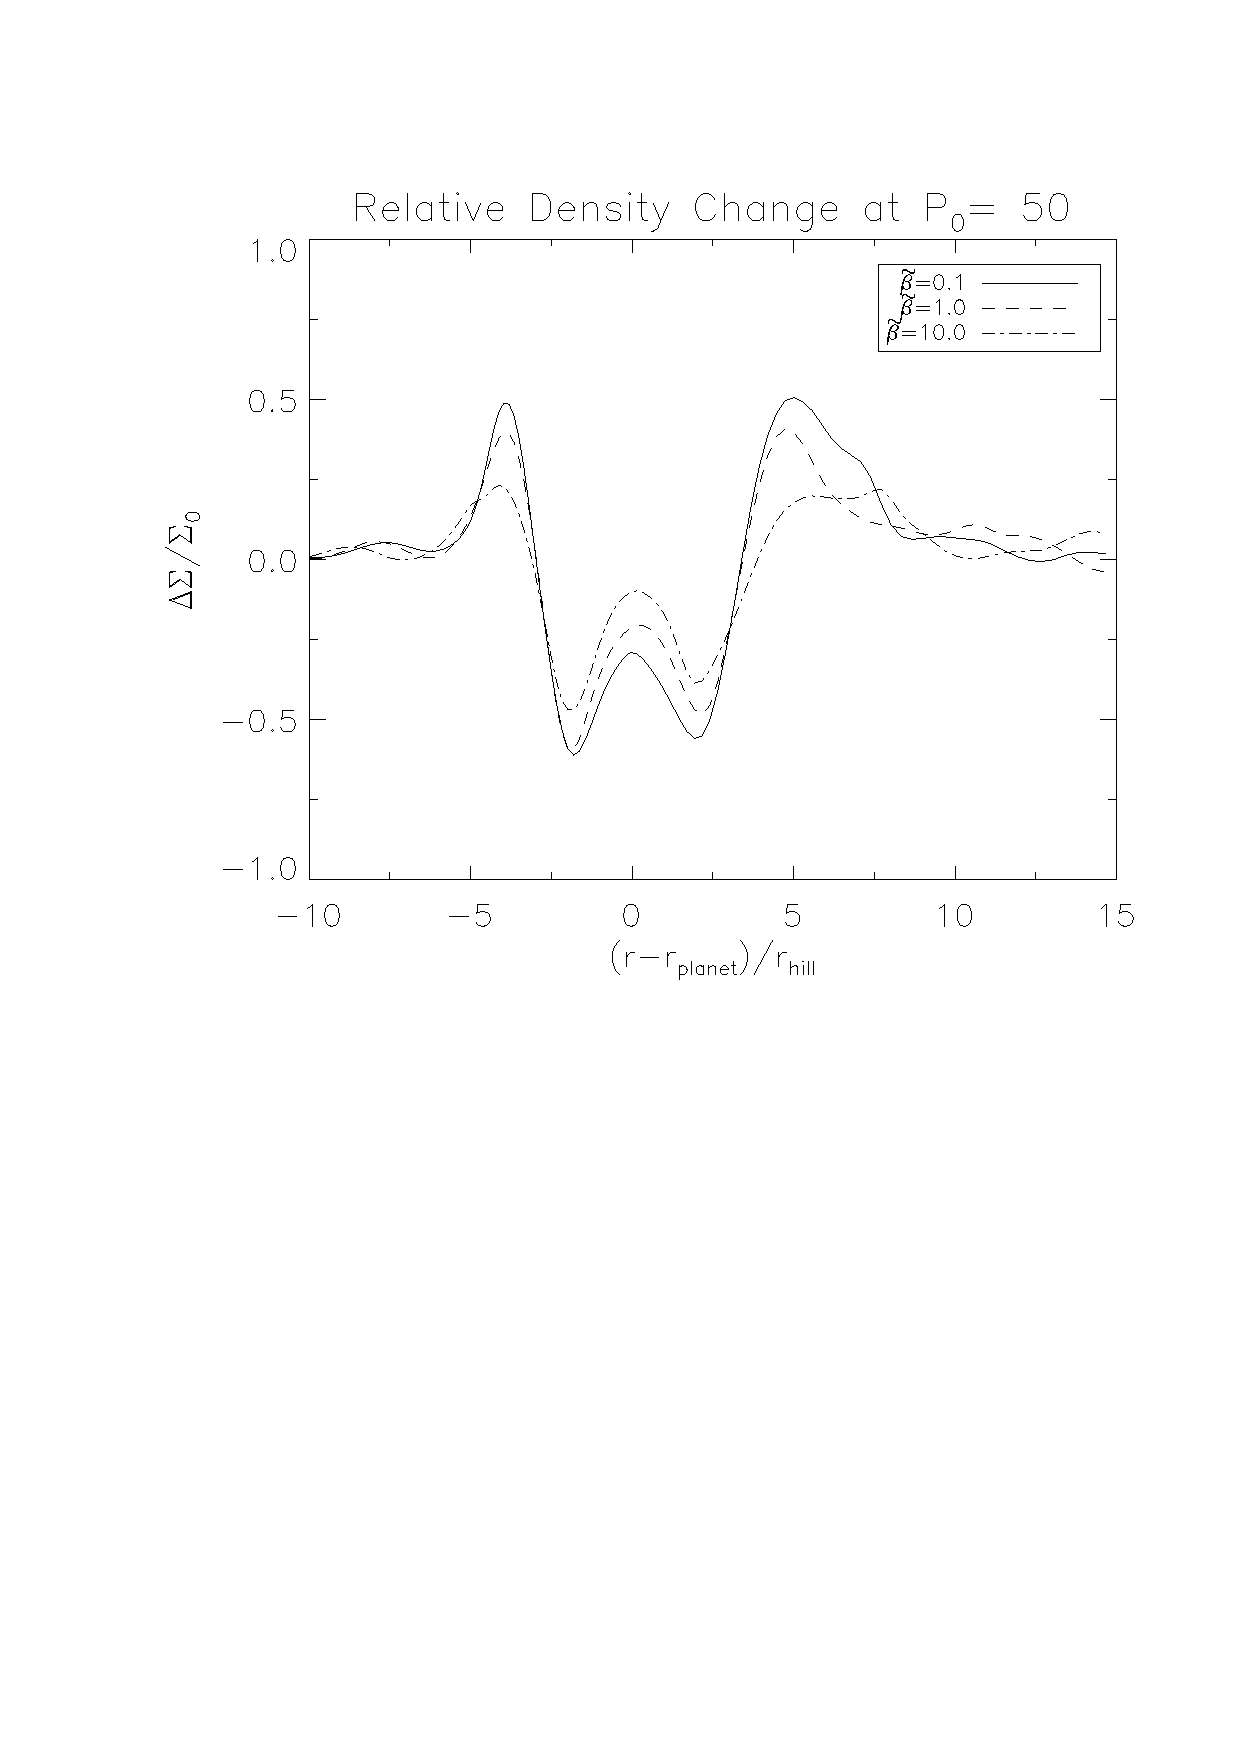
\includegraphics[width=\textwidth]{Posterfig_Density}
                    \end{minipage}
                    \hfill
                    \begin{minipage}{0.49\textwidth}
                      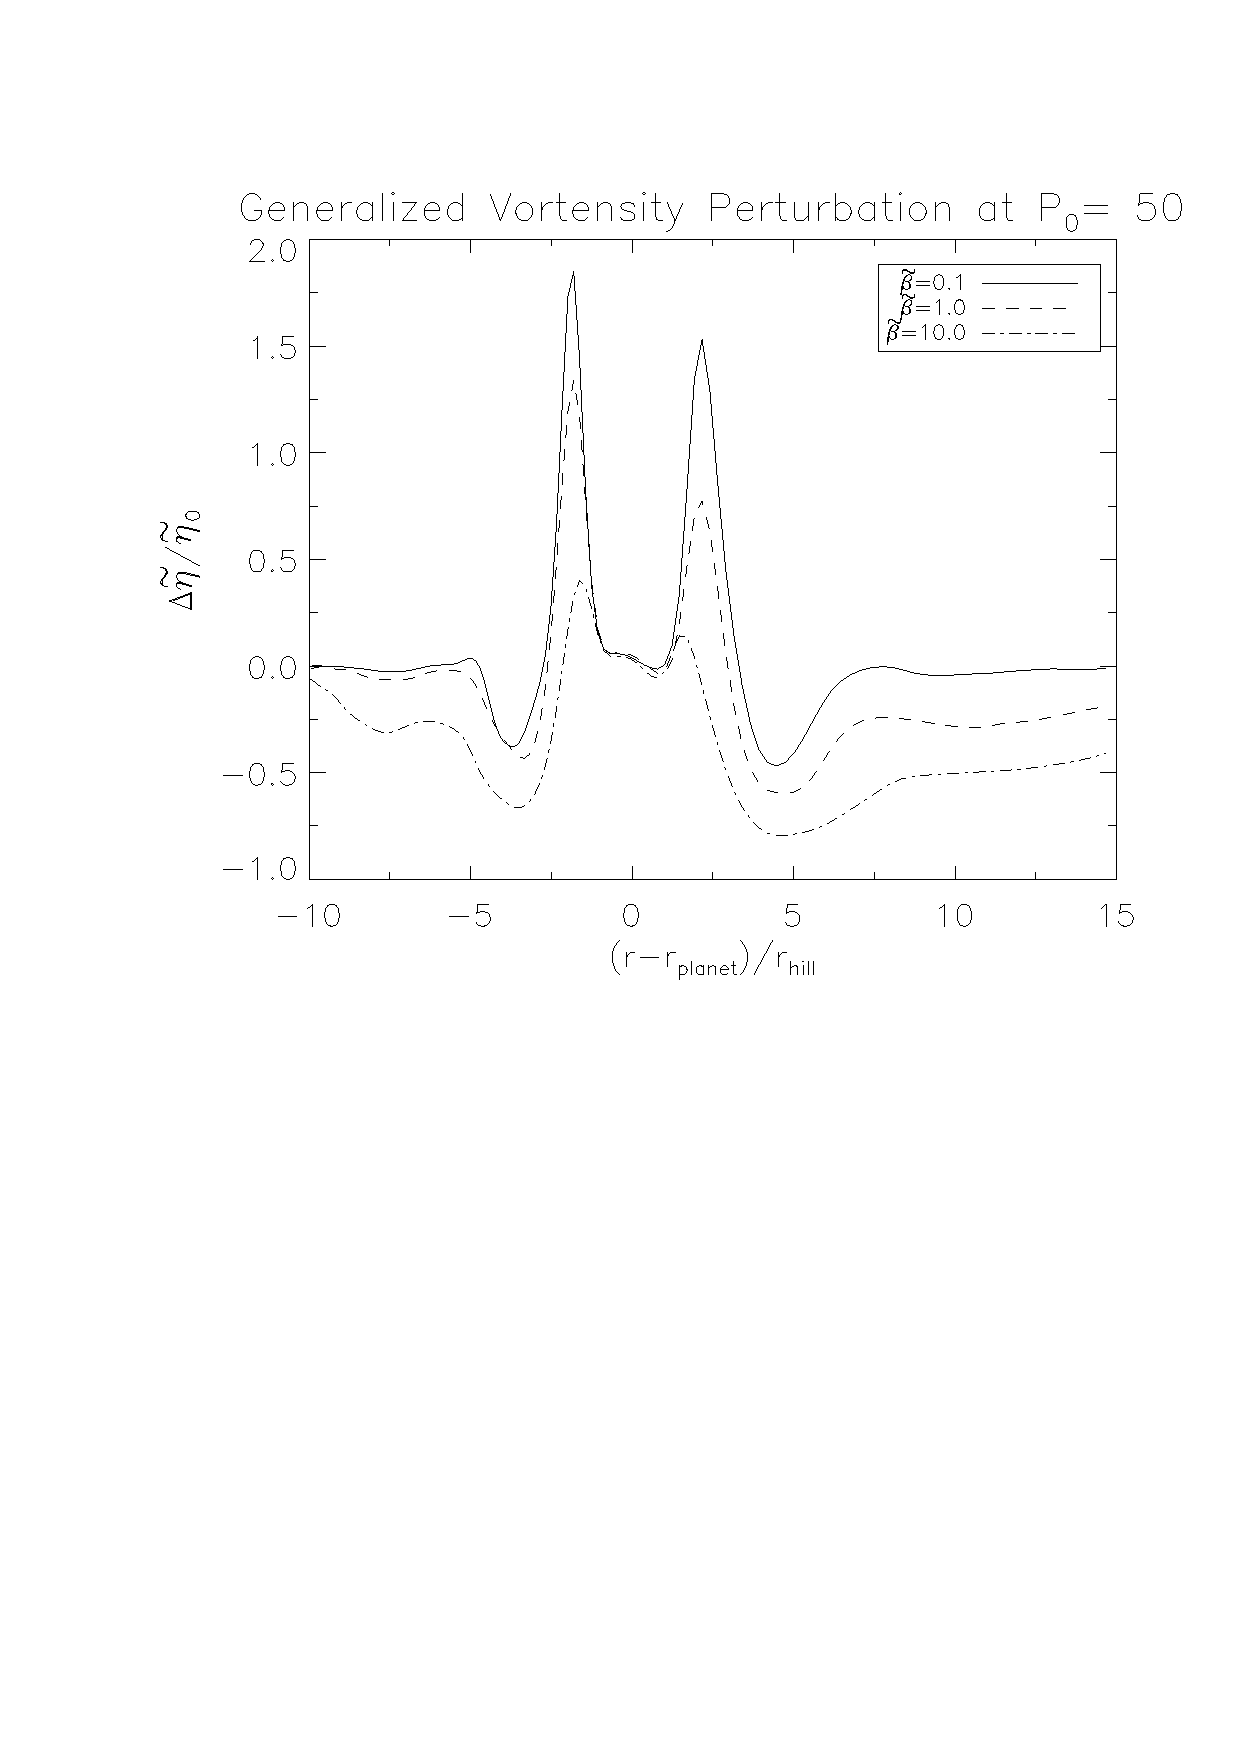
\includegraphics[width=\textwidth]{Posterfig_Vortensity}
                    \end{minipage}
                    \hfill
                  \end{figure}

                  \begin{figure}
                    \centering
                    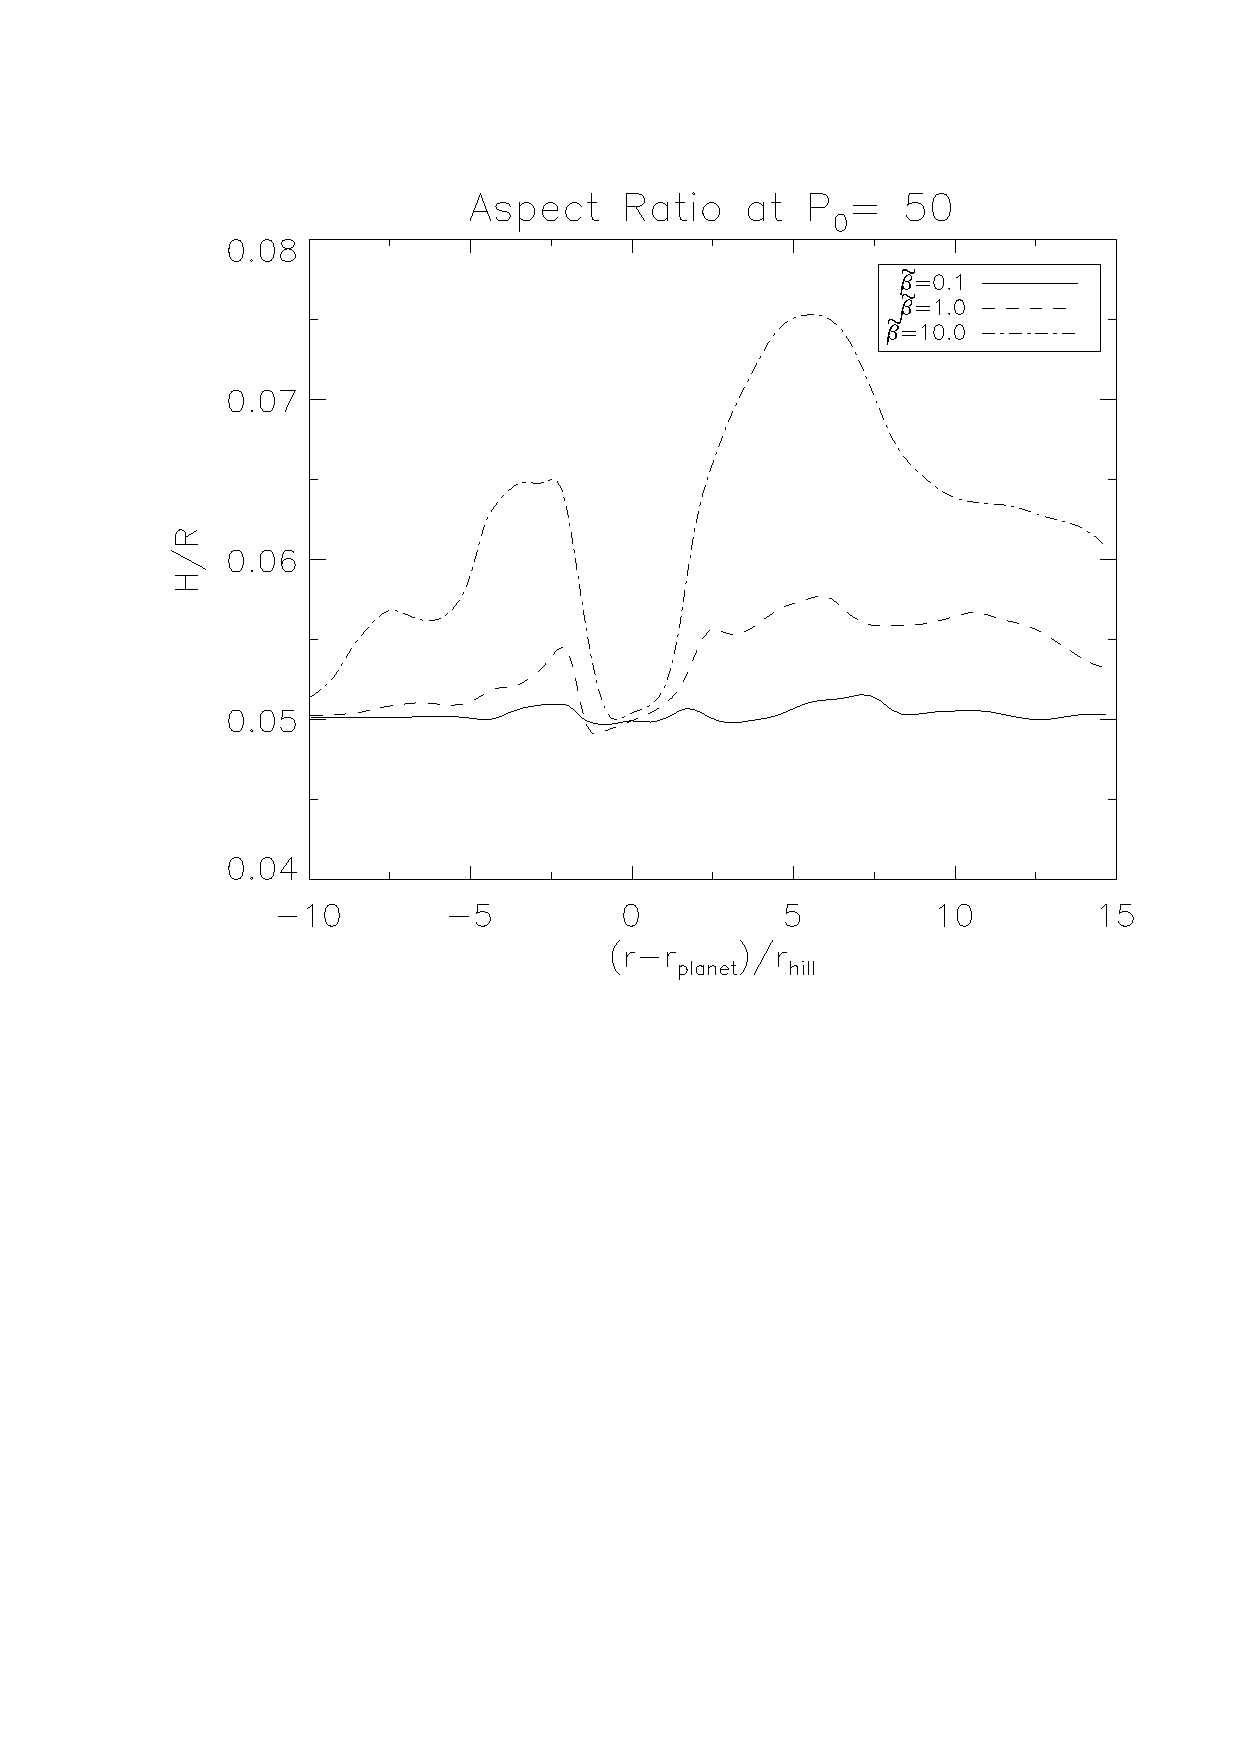
\includegraphics[width=0.5\textwidth]{Posterfig_HR}
                  \end{figure}
                  
            \end{block}
            
            \vfill

            \begin{block}{{\Large Linear stability}}
              \justifying
                  {\bf plot of growth rate v.s m for different beta,
                    or table. 2D density plot showing development of
                    vortex, for different beta}

                   \begin{figure}
                    \centering
                    \hfill
                    \begin{minipage}{0.45\textwidth}
                      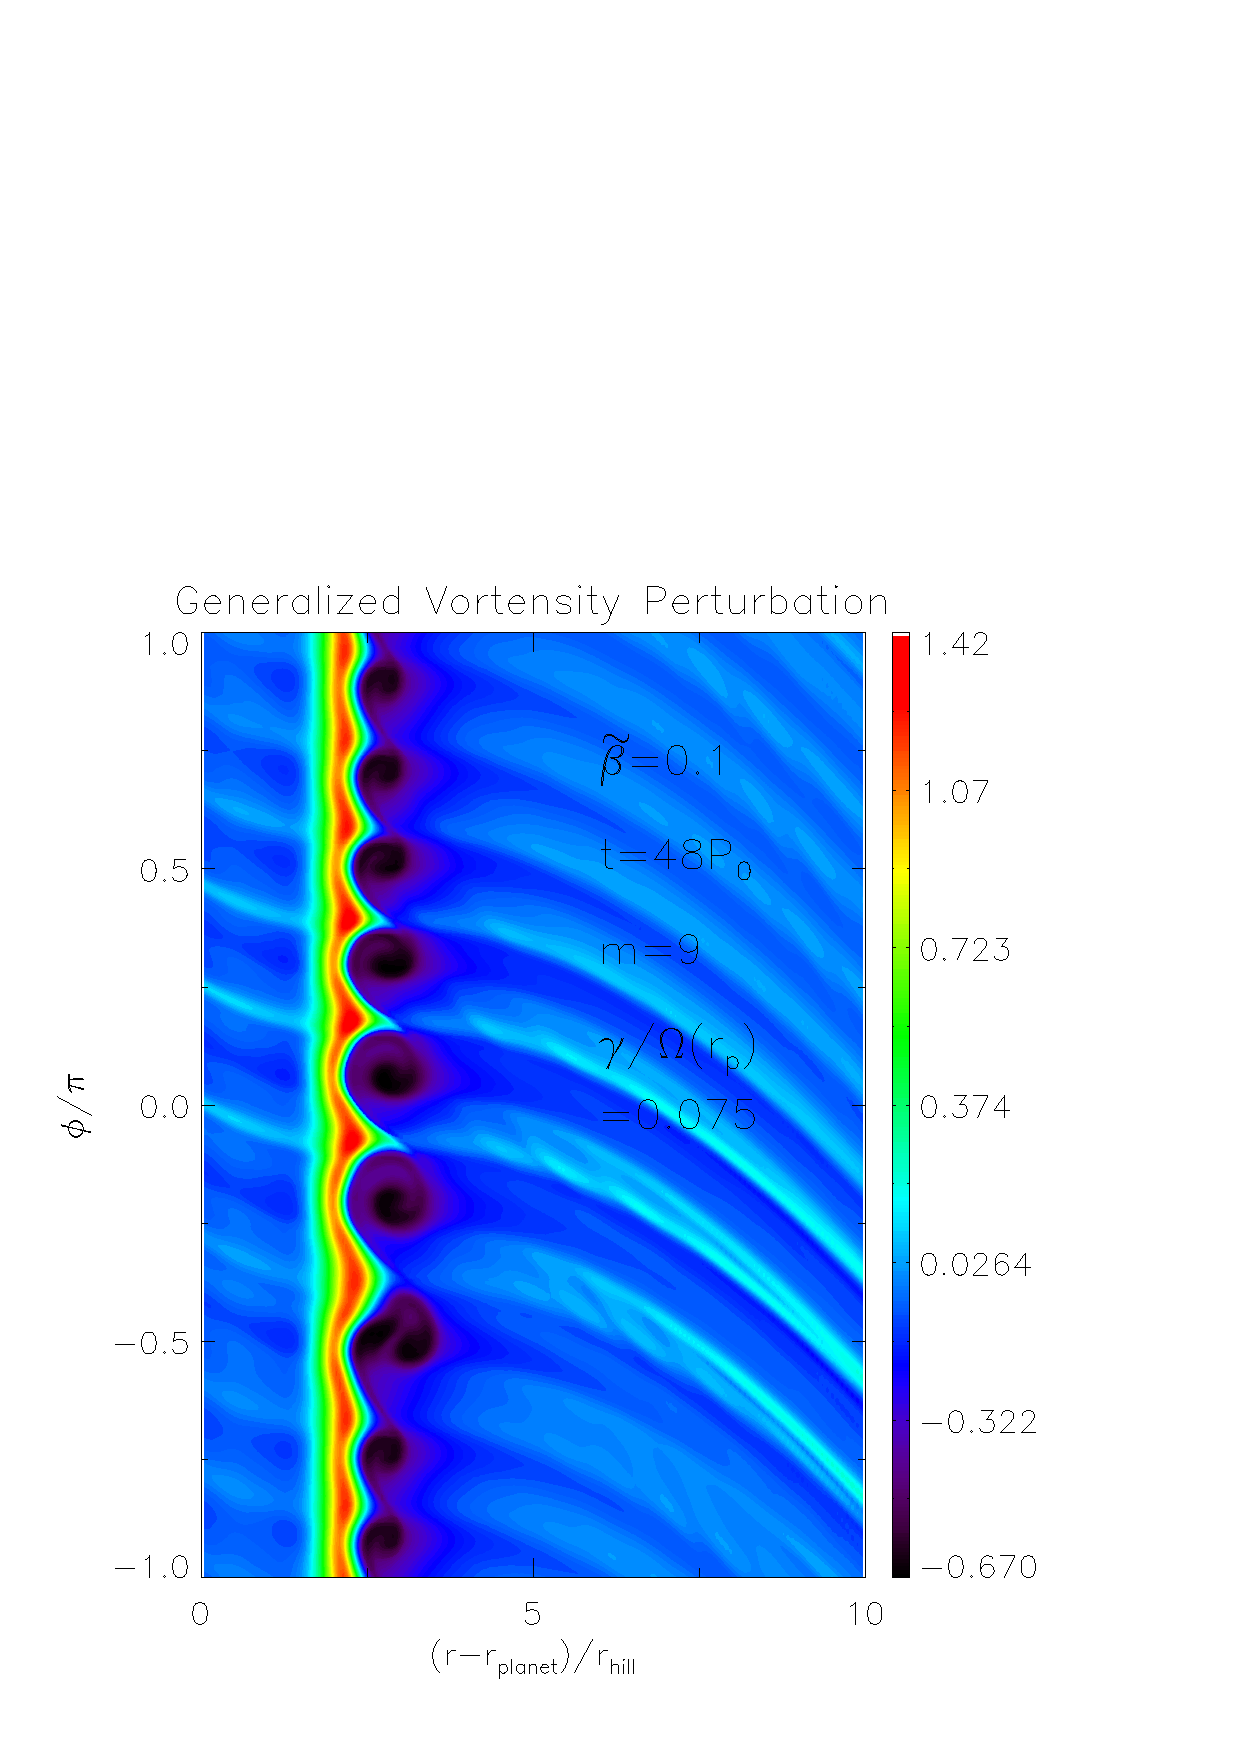
\includegraphics[width=\textwidth]{Posterfig_lowb}
                    \end{minipage}
                    \hfill
                    \begin{minipage}{0.45\textwidth}
                      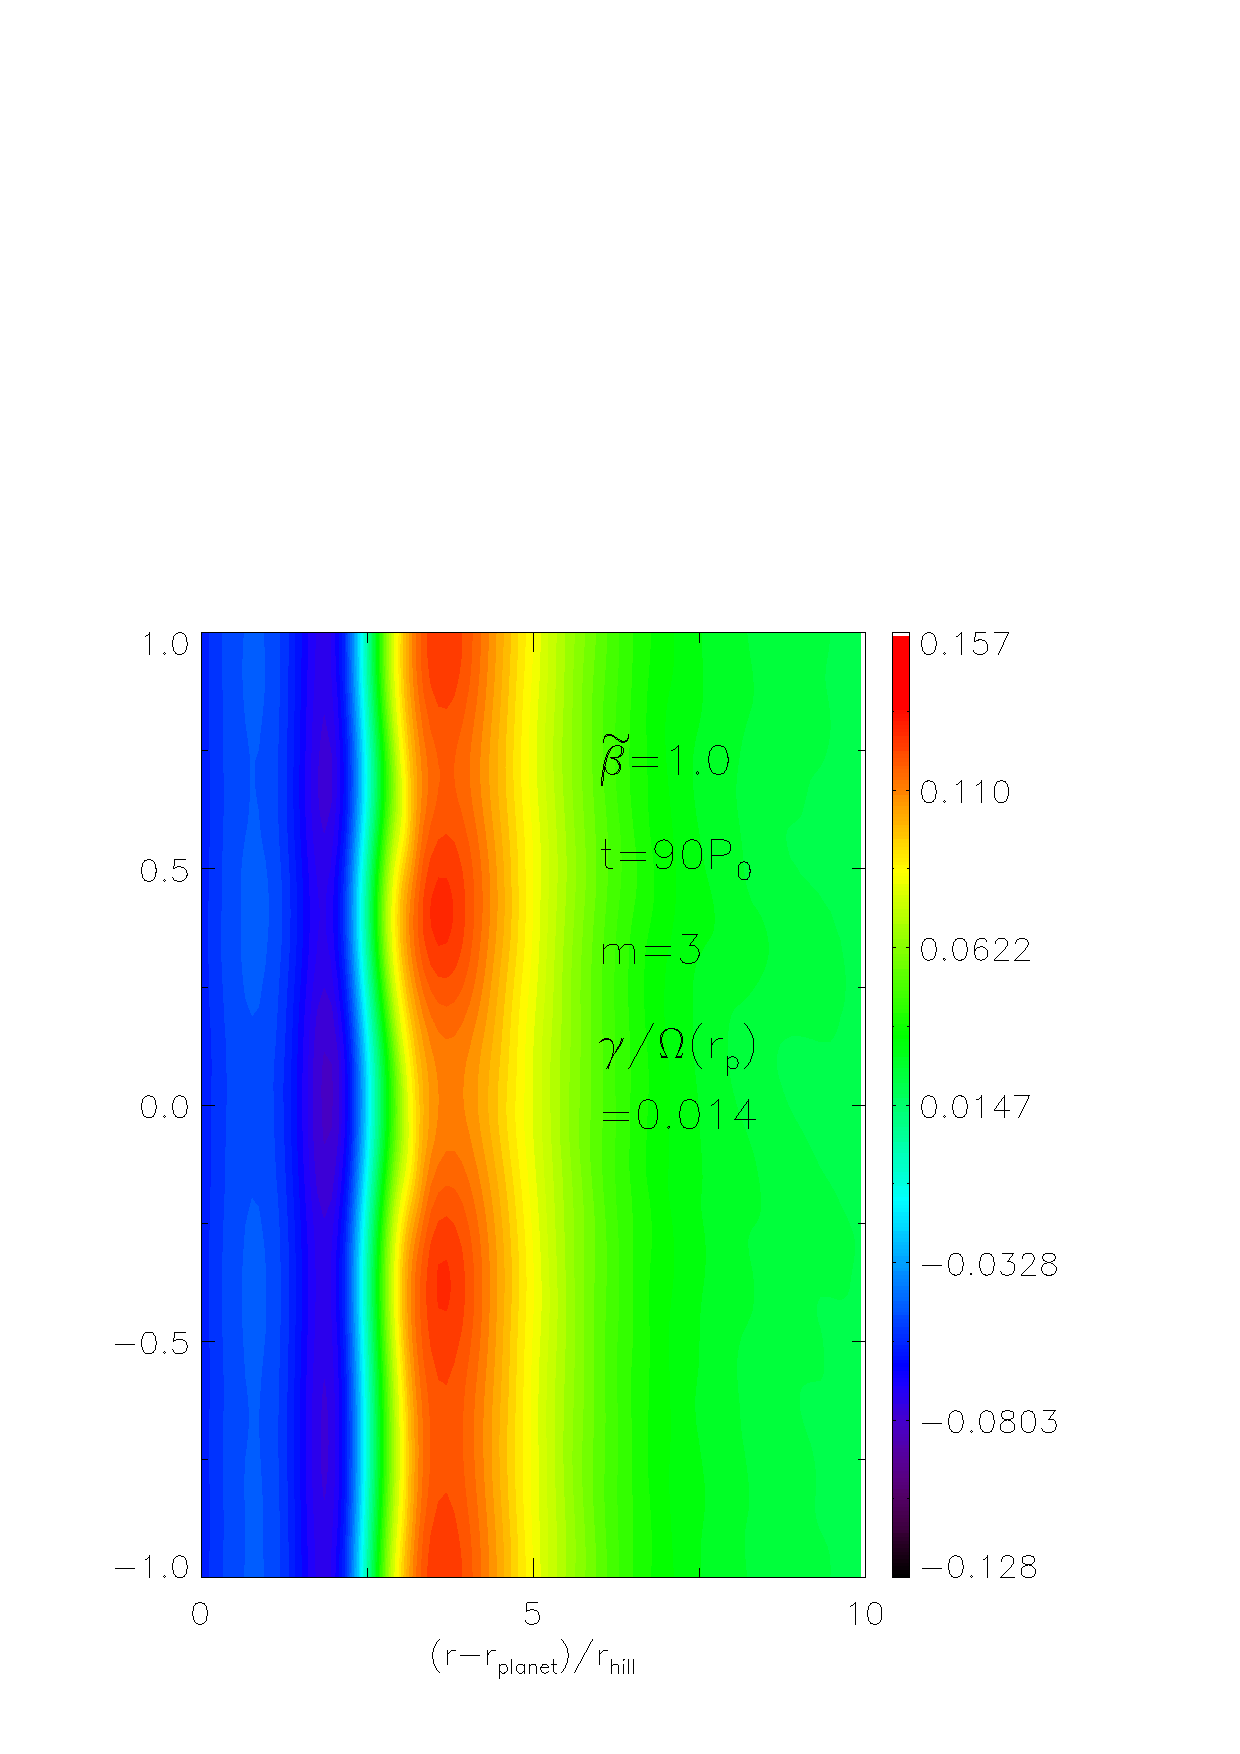
\includegraphics[width=\textwidth]{Posterfig_medb}
                    \end{minipage}
                    \hfill
                  \end{figure}

                   \begin{table}
                     \hfill
                     \begin{minipage}{0.45\textwidth}
                       \begin{tabularx}{\textwidth}{l*{5}{R}} \toprule \addlinespace[10pt]
                         \multicolumn{6}{c}{$\tilde{\beta}=0.1$} \\ \midrule
                         m                    & 1 & 2 & 3 & 4 & 5  \\ 
                         $\gamma/\Omega(r_o)$ & 1 & 2 & 3 & 4 & 5   \\ \bottomrule
                       \end{tabularx}
                     \end{minipage}
                     \hfill
                     \begin{minipage}{0.45\textwidth}
                       \begin{tabularx}{\textwidth}{l*{5}{R}} \toprule \addlinespace[10pt]
                         \multicolumn{6}{c}{$\tilde{\beta}=1.0$} \\ \midrule
                         m                    & 1 & 2 & 3 & 4 & 5  \\ 
                         $\gamma/\Omega(r_o)$ & 1 & 2 & 3 & 4 & 5   \\ \bottomrule
                       \end{tabularx}
                     \end{minipage}
                     \hfill
                   \end{table}

                  
            \end{block}
            \vfill
          }
        \end{minipage}
      \end{beamercolorbox}
    \end{column}
    % ---------------------------------------------------------%
    % end the column
    
    % ---------------------------------------------------------%
    % Set up a column 
    \begin{column}{.49\textwidth}
      \begin{beamercolorbox}[center,wd=\textwidth]{postercolumn}
        \begin{minipage}[T]{.95\textwidth} % tweaks the width, makes a new \textwidth
          \parbox[t][\columnheight]{\textwidth}{ % must be some better way to set the the height, width and textwidth simultaneously
            % Since all columns are the same length, it is all nice and tidy.  You have to get the height empirically
            % ---------------------------------------------------------%
            % fill each column with content
            
            \begin{block}{\Large{Linear stability Cont.}}
              \justifying
              \begin{figure}
                \centering
                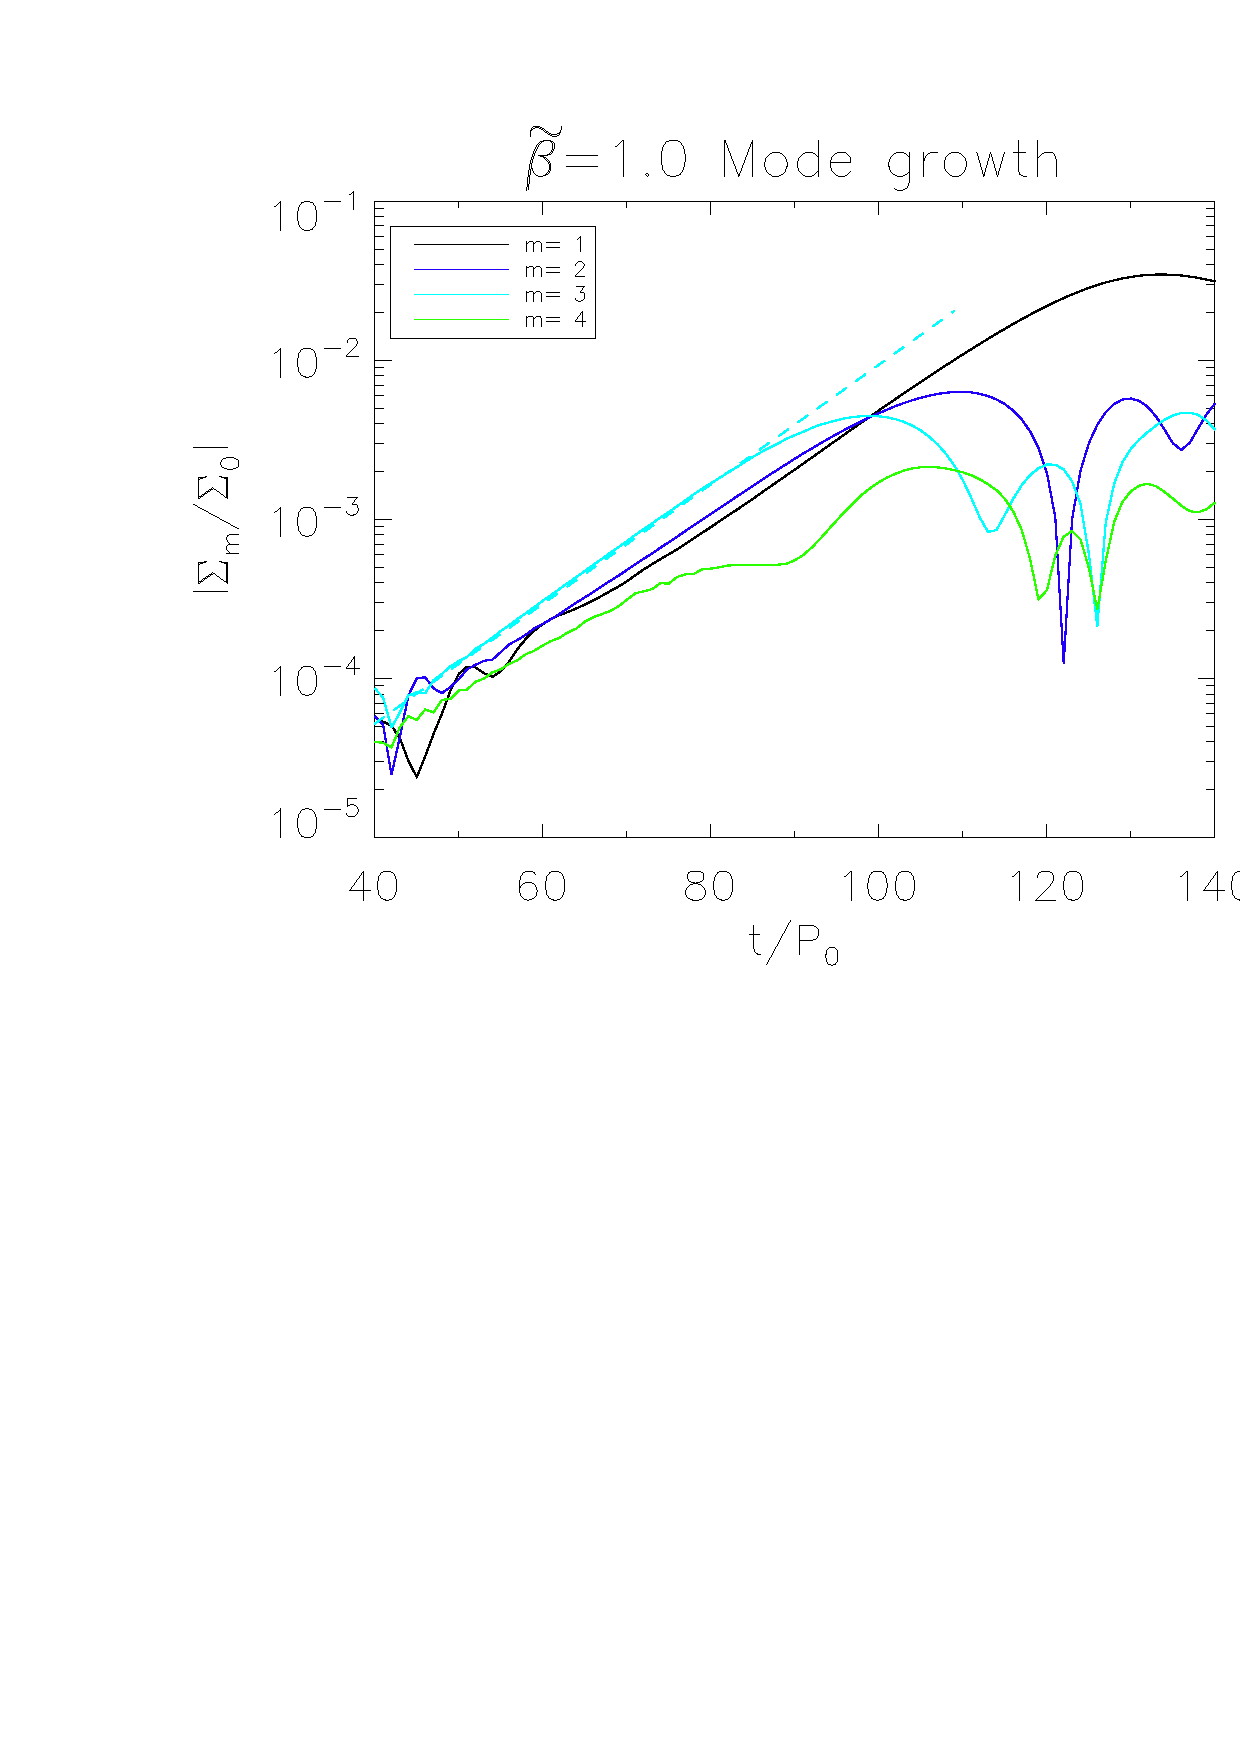
\includegraphics[width=\textwidth]{Posterfig_Growth}
              \end{figure}
            \end{block}

            \vfill

            \begin{block}{\Large{Non-linear vortex evolution}}
              \justifying
                  {\bf `lifetime' plot of m=1 for diff beta, snapshots
                    (before, during, after vortex decay). quote rossby
                  number when vortices in quasi-steady state}

                  \begin{figure}
                    \centering
                    \includegraphics[width=\textwidth]{Posterfig_Lifetime_b}
                  \end{figure}

                  \begin{figure}
                    \centering
                    \hfill
                    \begin{minipage}{0.3\textwidth}
                      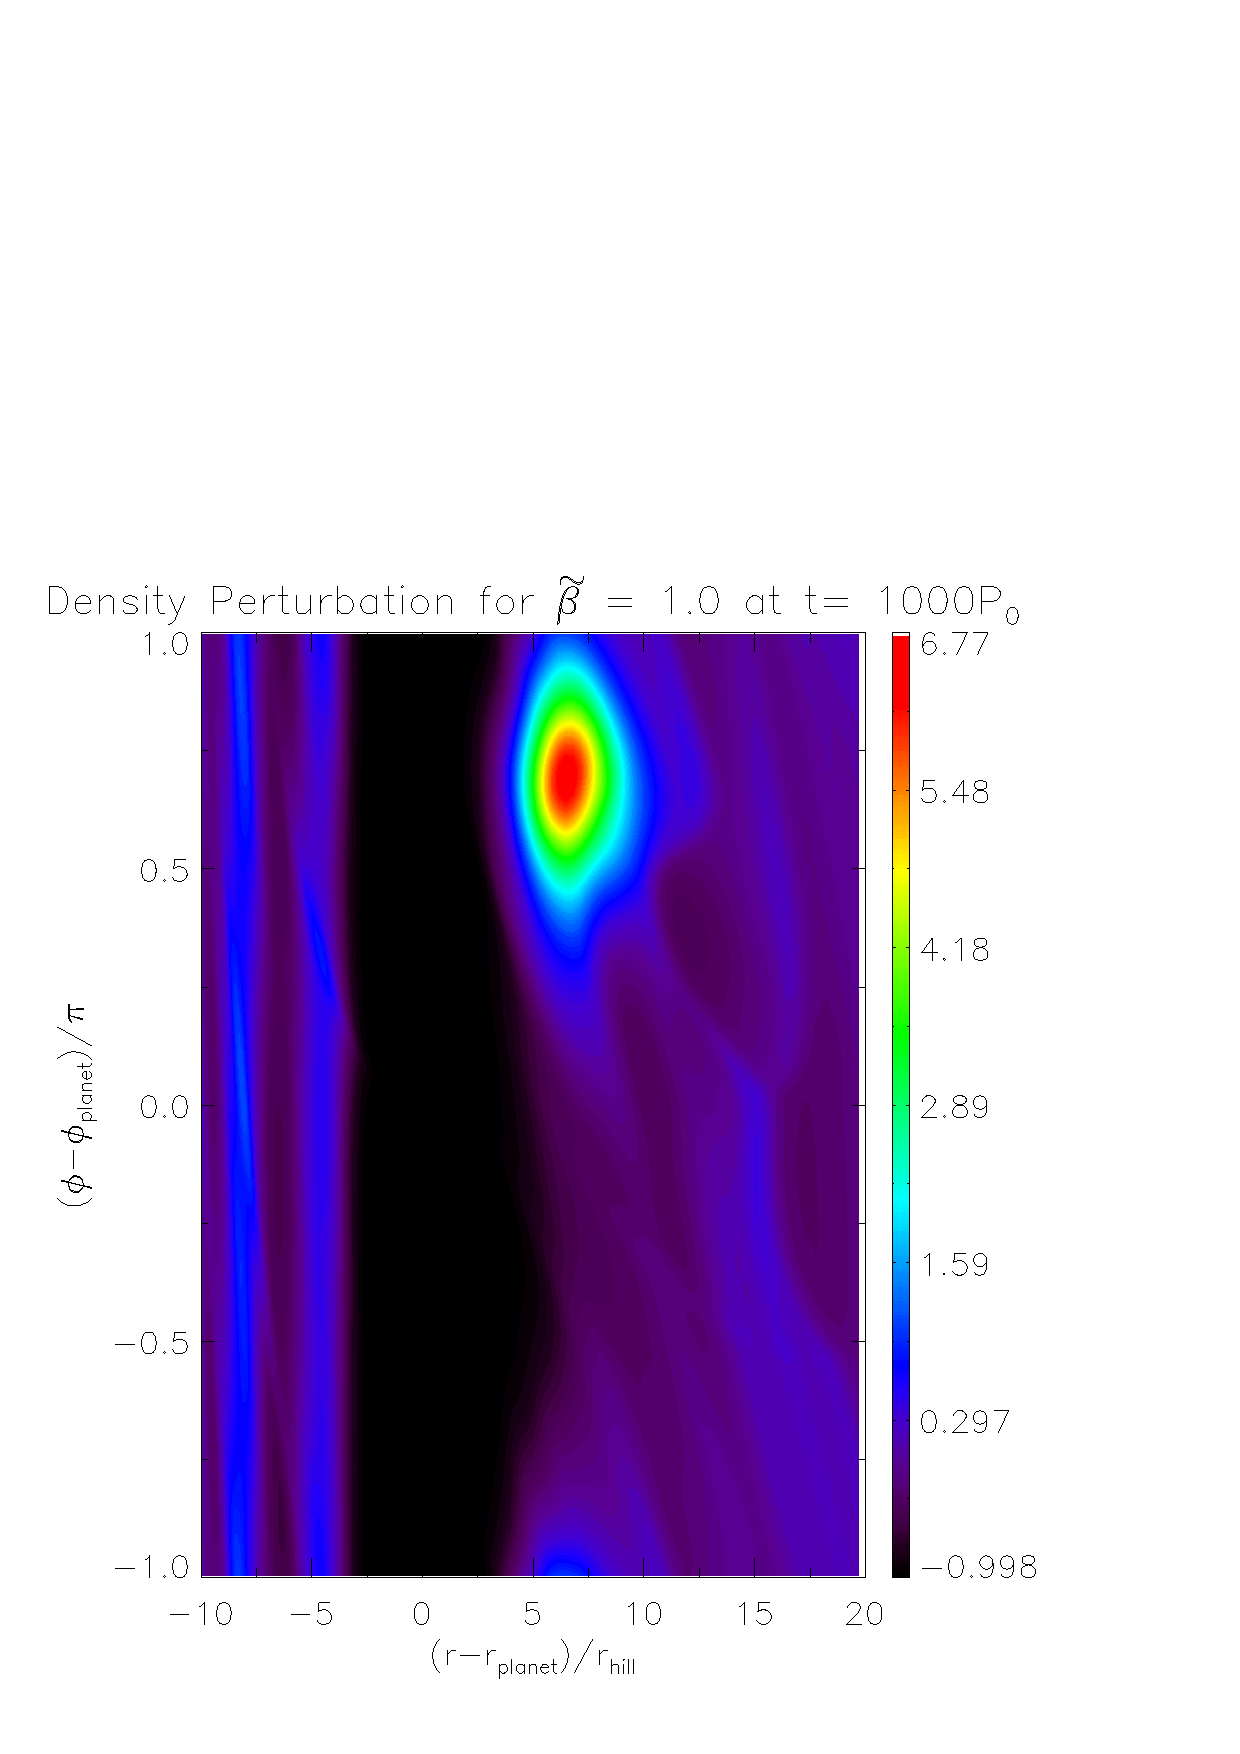
\includegraphics[width=\textwidth]{Posterfig_Before}
                      \caption{$Ro=-0.16$}
                    \end{minipage}
                    \hfill
                    \begin{minipage}{0.3\textwidth}
                      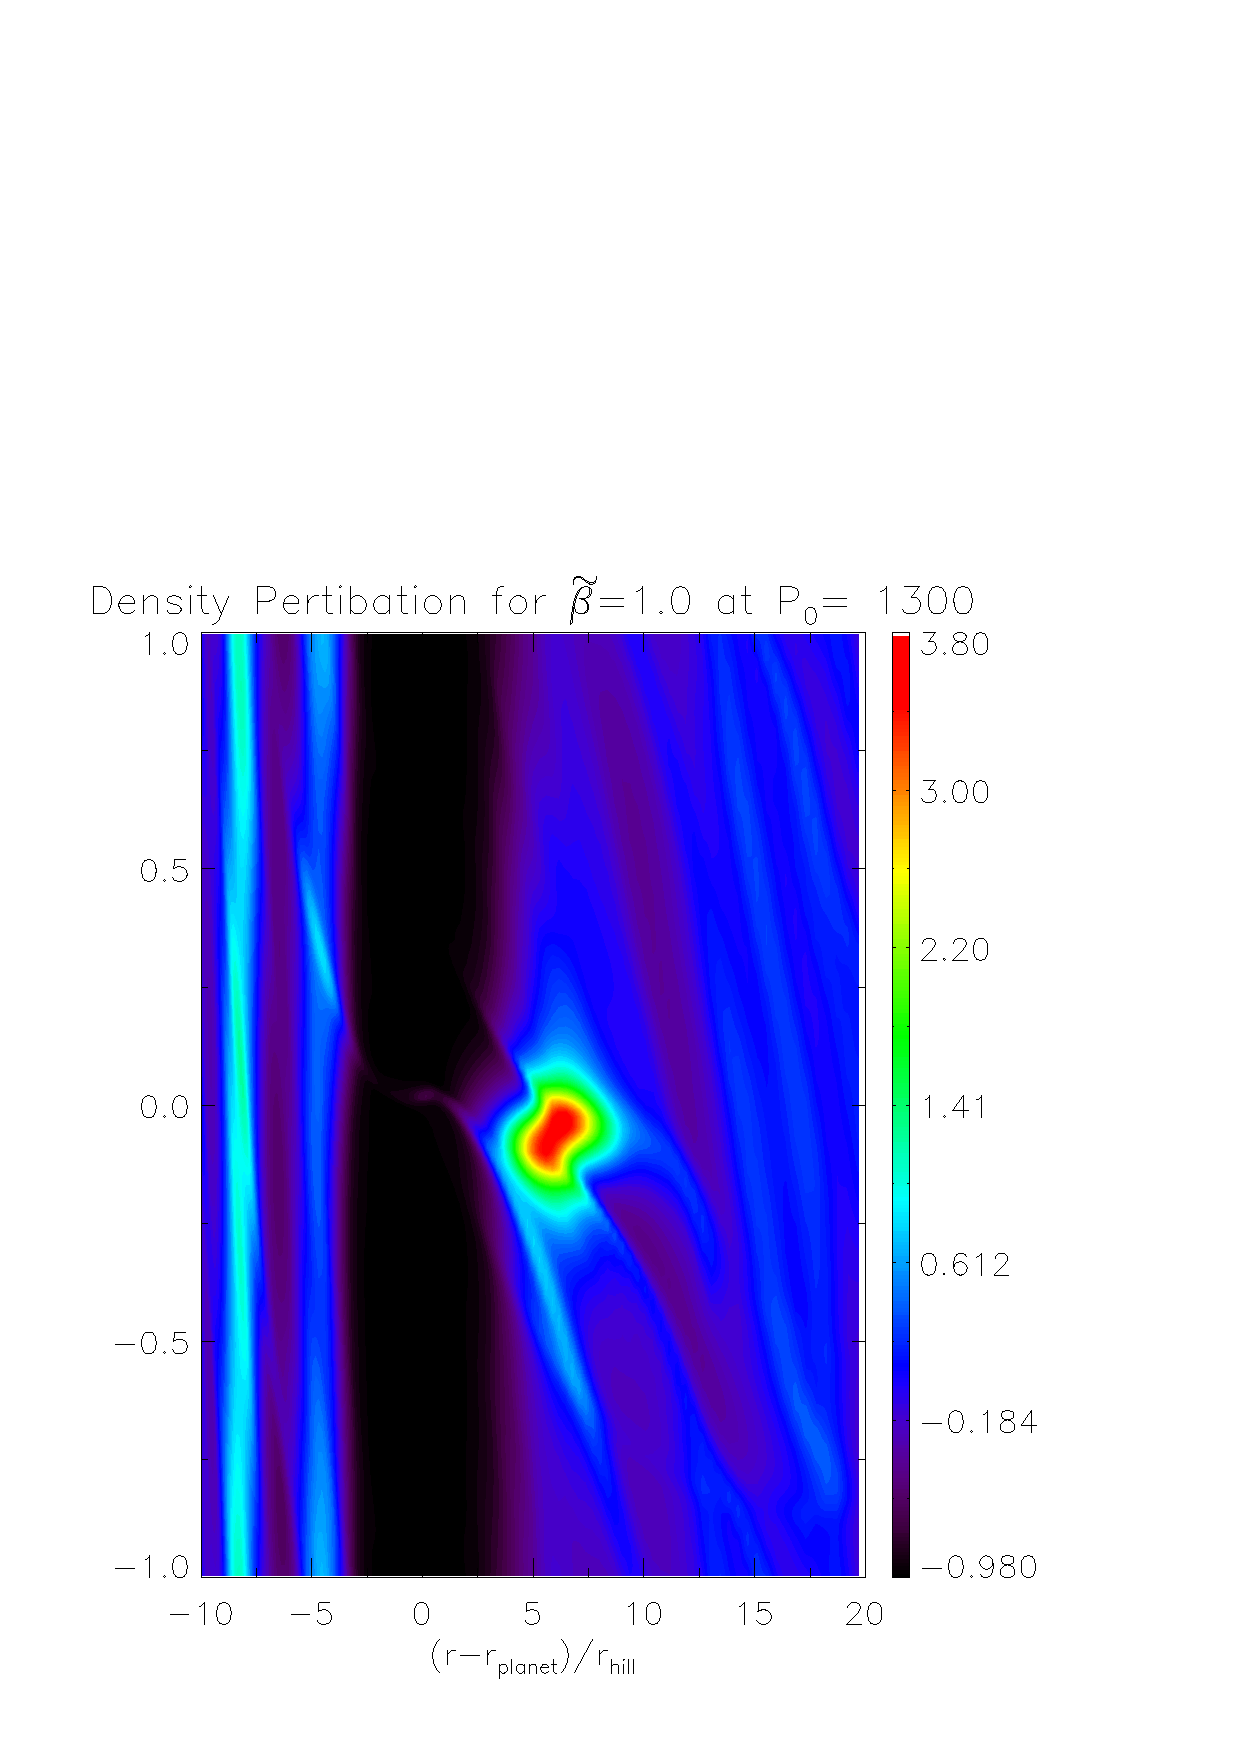
\includegraphics[width=\textwidth]{Posterfig_During}
                      \caption{$Ro=-0.43$}
                    \end{minipage}
                    \hfill
                    \begin{minipage}{0.3\textwidth}
                      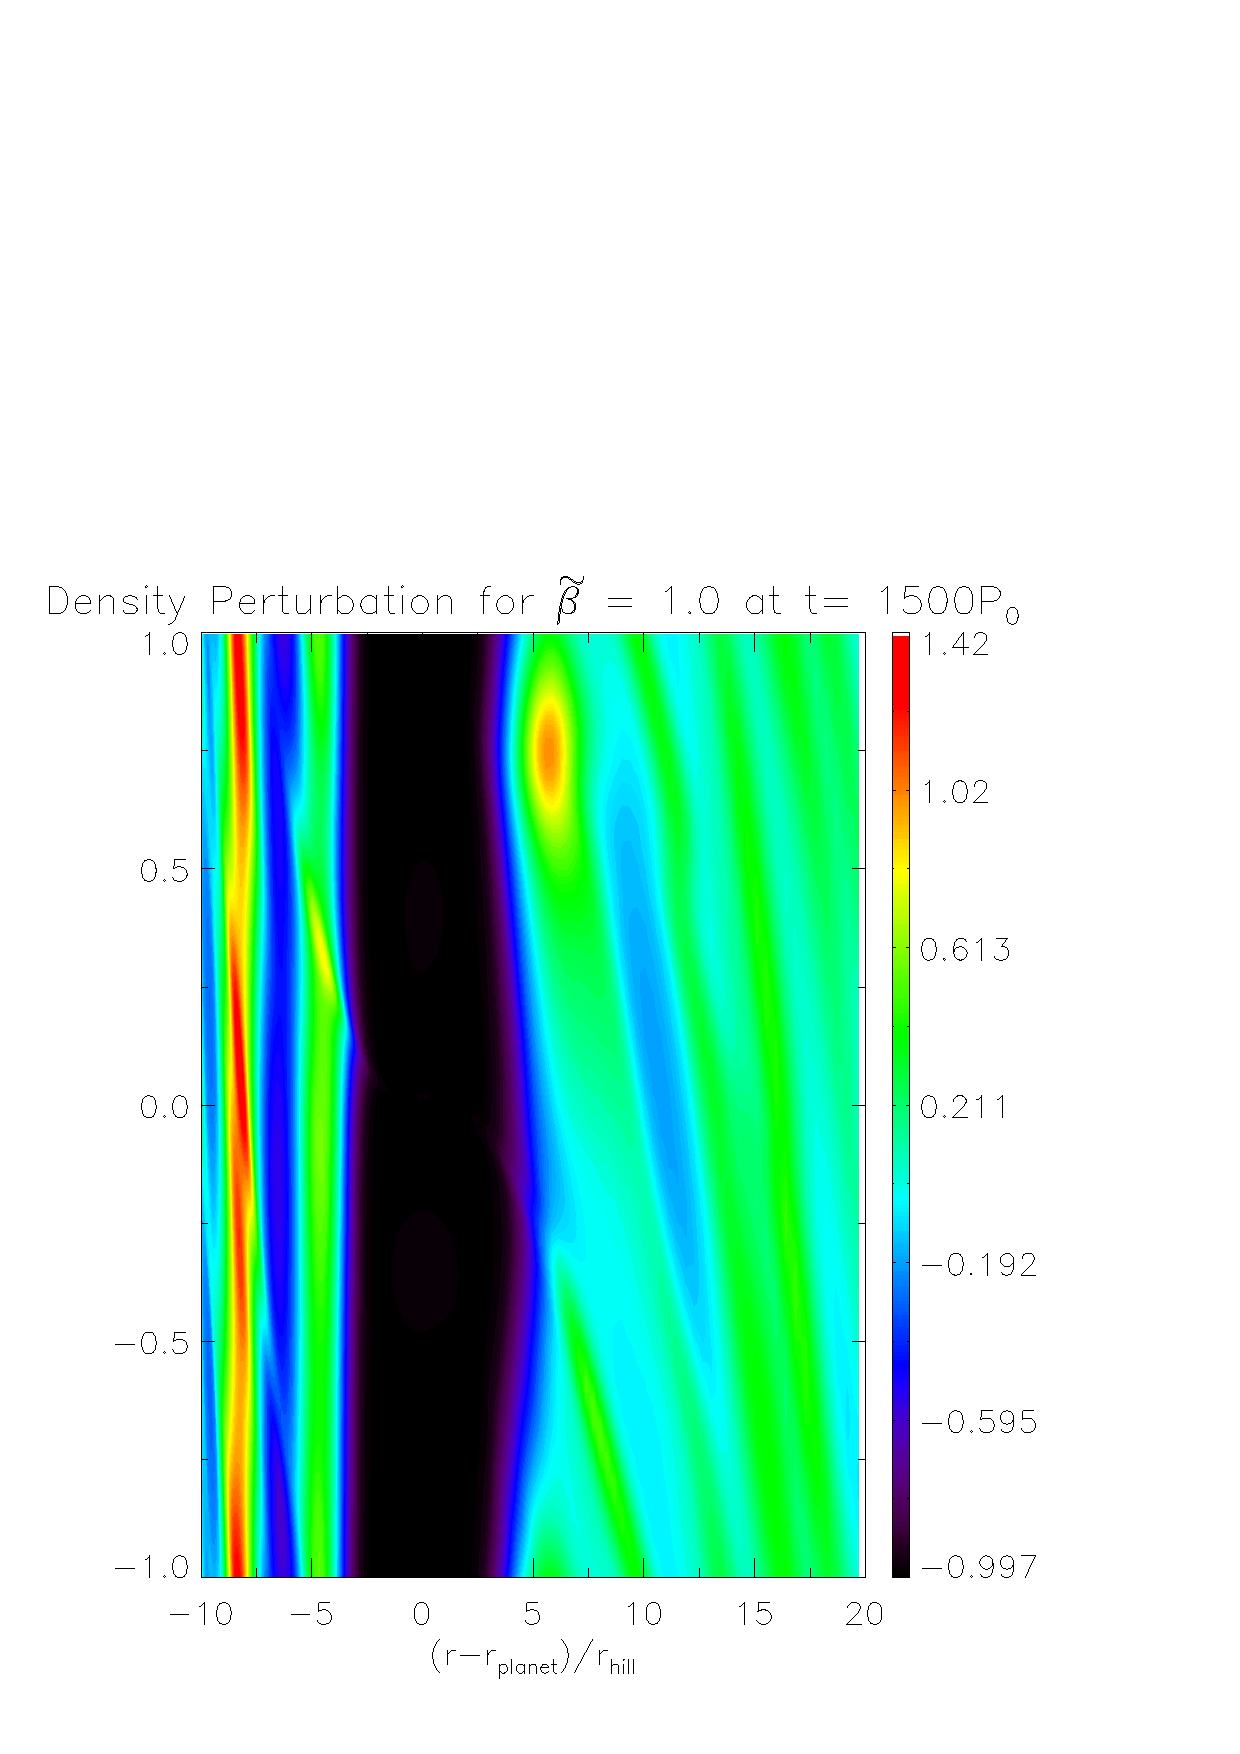
\includegraphics[width=\textwidth]{Posterfig_After}
                      \caption{$Ro=-0.10$}
                    \end{minipage}
                    \hfill
                  \end{figure}

            \end{block}
            \vfill
    
            \begin{block}{{\Large Conclusions so far}}\justifying
              {\large{\bf
                  
                }
              }
              \vfill
            \end{block}
          }
          % ---------------------------------------------------------%
          % end the column
        \end{minipage}
      \end{beamercolorbox}
    \end{column}
    % ---------------------------------------------------------%
    % end the column
  \end{columns}
  \vskip1ex
  %\tiny\hfill\textcolor{ta2gray}{Created with \LaTeX \texttt{beamerposter}  \url{http://www-i6.informatik.rwth-aachen.de/~dreuw/latexbeamerposter.php}}
  %% \tiny\hfill{Created with \LaTeX \texttt{beamerposter}  \url{http://www-i6.informatik.rwth-aachen.de/~dreuw/latexbeamerposter.php} \hskip1em}
\end{frame}
\end{document}


%%%%%%%%%%%%%%%%%%%%%%%%%%%%%%%%%%%%%%%%%%%%%%%%%%%%%%%%%%%%%%%%%%%%%%%%%%%%%%%%%%%%%%%%%%%%%%%%%%%%
%%% Local Variables: 
%%% mode: latex
%%% TeX-PDF-mode: t
%%% End:
